\documentclass{report}
\usepackage[margin=1in, paperwidth=8.5in, paperheight=11in]{geometry}
%Math packages%
\usepackage{amsmath}
\usepackage{amsthm}
%Spacing%
\usepackage{setspace}
\onehalfspacing
%Lecture number%
\newcommand{\lectureNum}{16}
%Variables - Date and Course%
\newcommand{\curDate}{March 2, 2017}
\newcommand{\course}{CS 241}
\newcommand{\instructor}{Kevin Lanctot}
%Defining the example tag%
%\theoremstyle{definition}%
\newtheorem{ex}{Example}[section]
%Setting counter given the lecture number%
\setcounter{chapter}{\lectureNum{}}
%Package to insert code%
\usepackage{listings}
\usepackage{courier}
\usepackage{xcolor}
\lstset { %
    tabsize=2,
    breaklines=true,
    language=C++,
    backgroundcolor=\color{blue!8}, % set backgroundcolor
    basicstyle=\footnotesize\ttfamily,% basic font setting
}
%Package for images%
\usepackage{graphicx}

\begin{document}
%Note title%
\begin{center}
\begin{Large}
\textsc{\course{} | Lecture \lectureNum{}}
\end{Large}
\end{center} 
\noindent \textit{Bartosz Antczak} \hfill
\textit{Instructor: \instructor{}} \hfill
\textit{\curDate{}}
\rule{\textwidth}{0.4pt}
% Actual Notes%
\subsubsection{Remark}
Assignment 7 is out, and according to Prof. Lanctot, it's the hardest assignment to complete in the course. About 50\% of students won't finish it. Because of this, Prof. Lanctot will review parsing (which is the topic of assignment 7).
\subsection{Review of Parsing}
Parsing validates whether a given word in accepted for a particular context-free grammar. There's two types of parsing: top-down or bottom-up.
\subsubsection{Top-Down Parsing}
Start with our start state ($S$) and using the given derivation rules for our CFG, we can check if there exists a derivation from $S$ to the given word.
\begin{ex}
Top-down parsing on a particular CFG using the word `abywz'
\end{ex}
\begin{figure}[ht]
\begin{center}
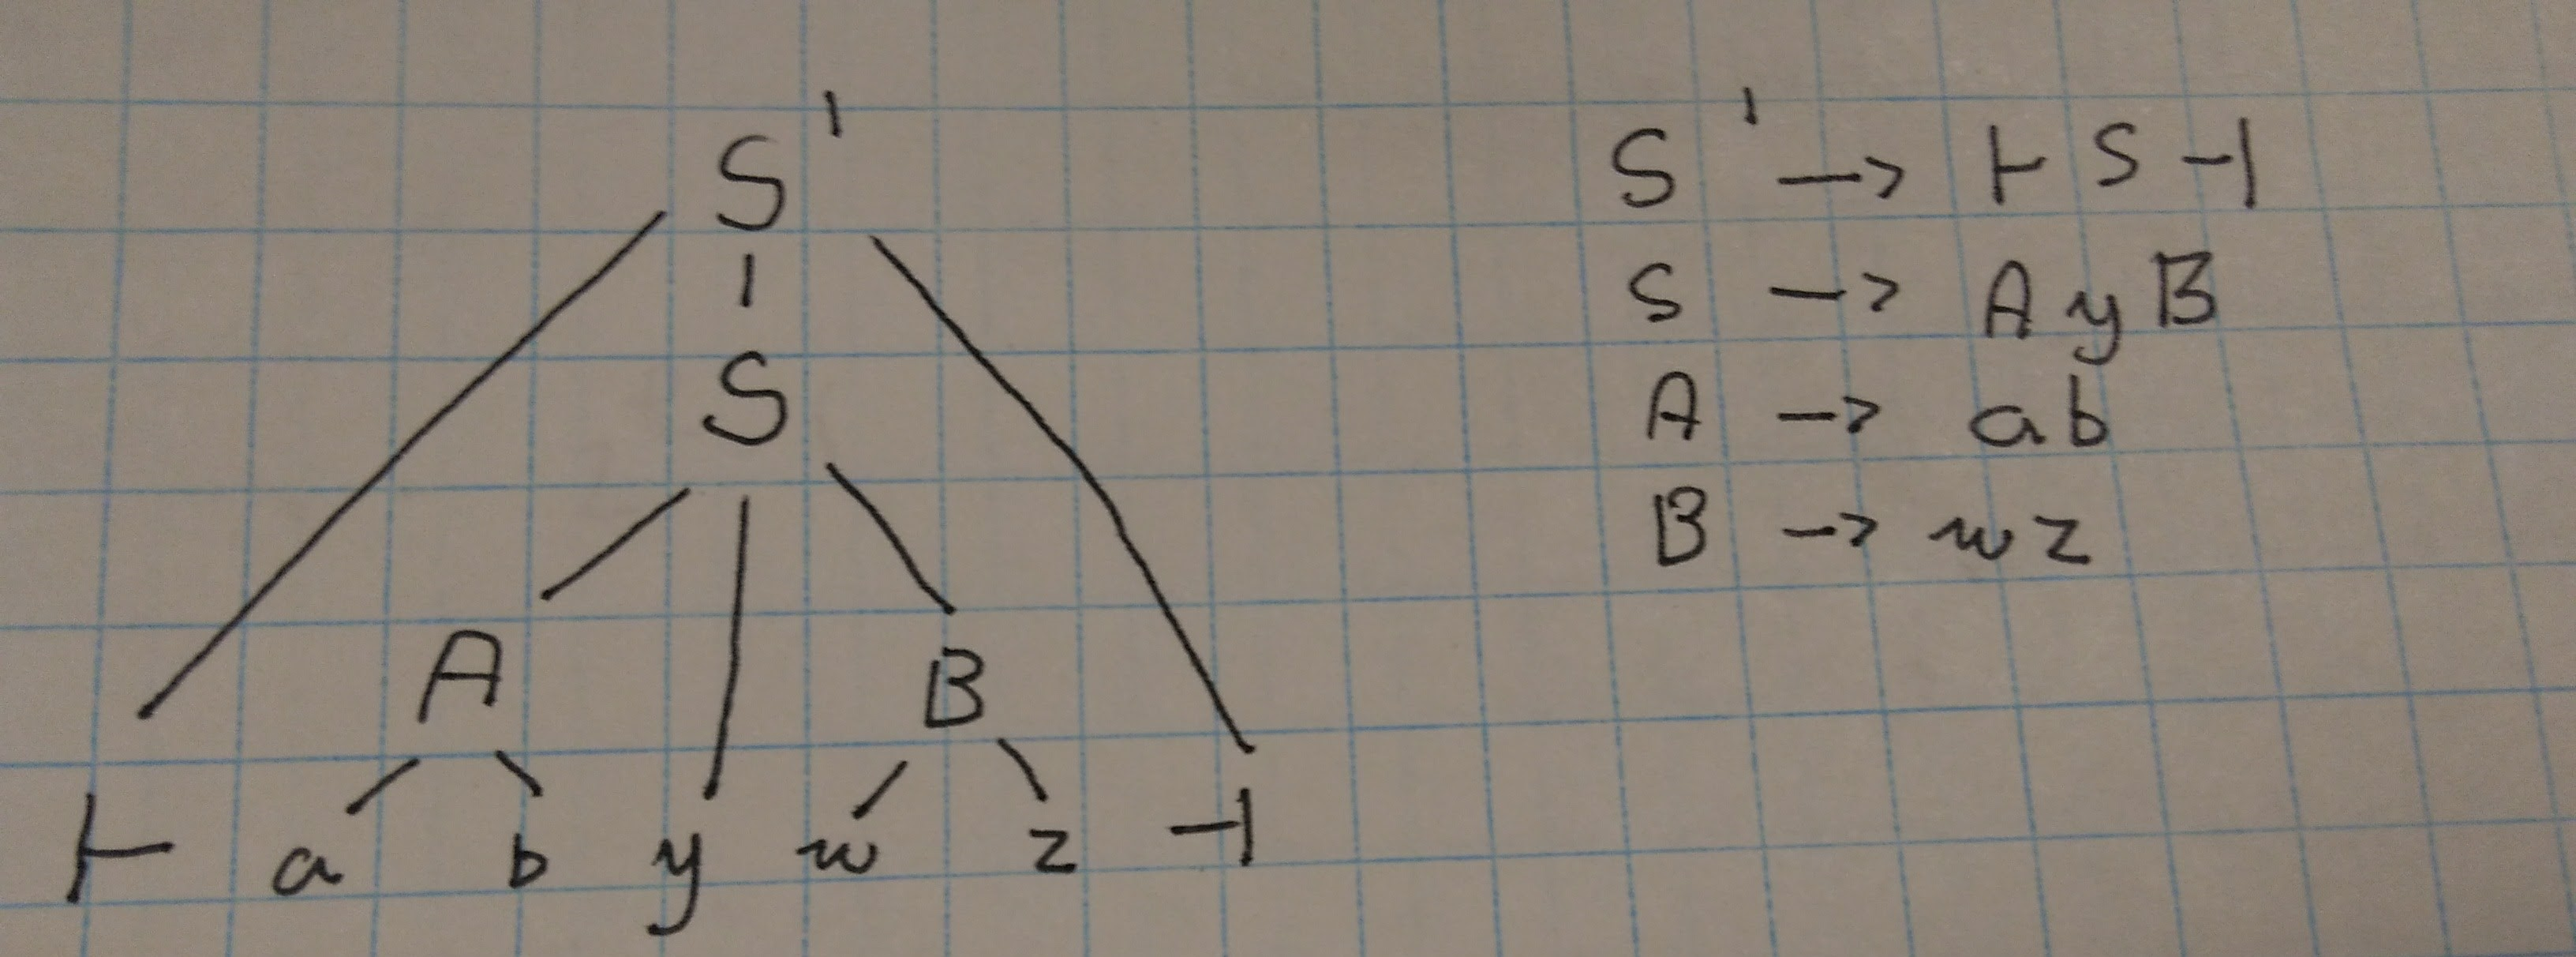
\includegraphics[scale=0.1]{top-down1.jpg}
\end{center}
\end{figure}
How can we determine which derivation rule to use? We use the implementation for top-down parsing, called LL(1) Parsing.
Before we implement LL(1) Parsing, we need to outline a couple of methods:
\begin{itemize}
\item \texttt{first($\alpha$)}: given a non-terminal $\alpha$, find all of the possible tokens that can be derived from it. It returns the first character from those tokens:
\begin{figure}[ht]
\begin{center}
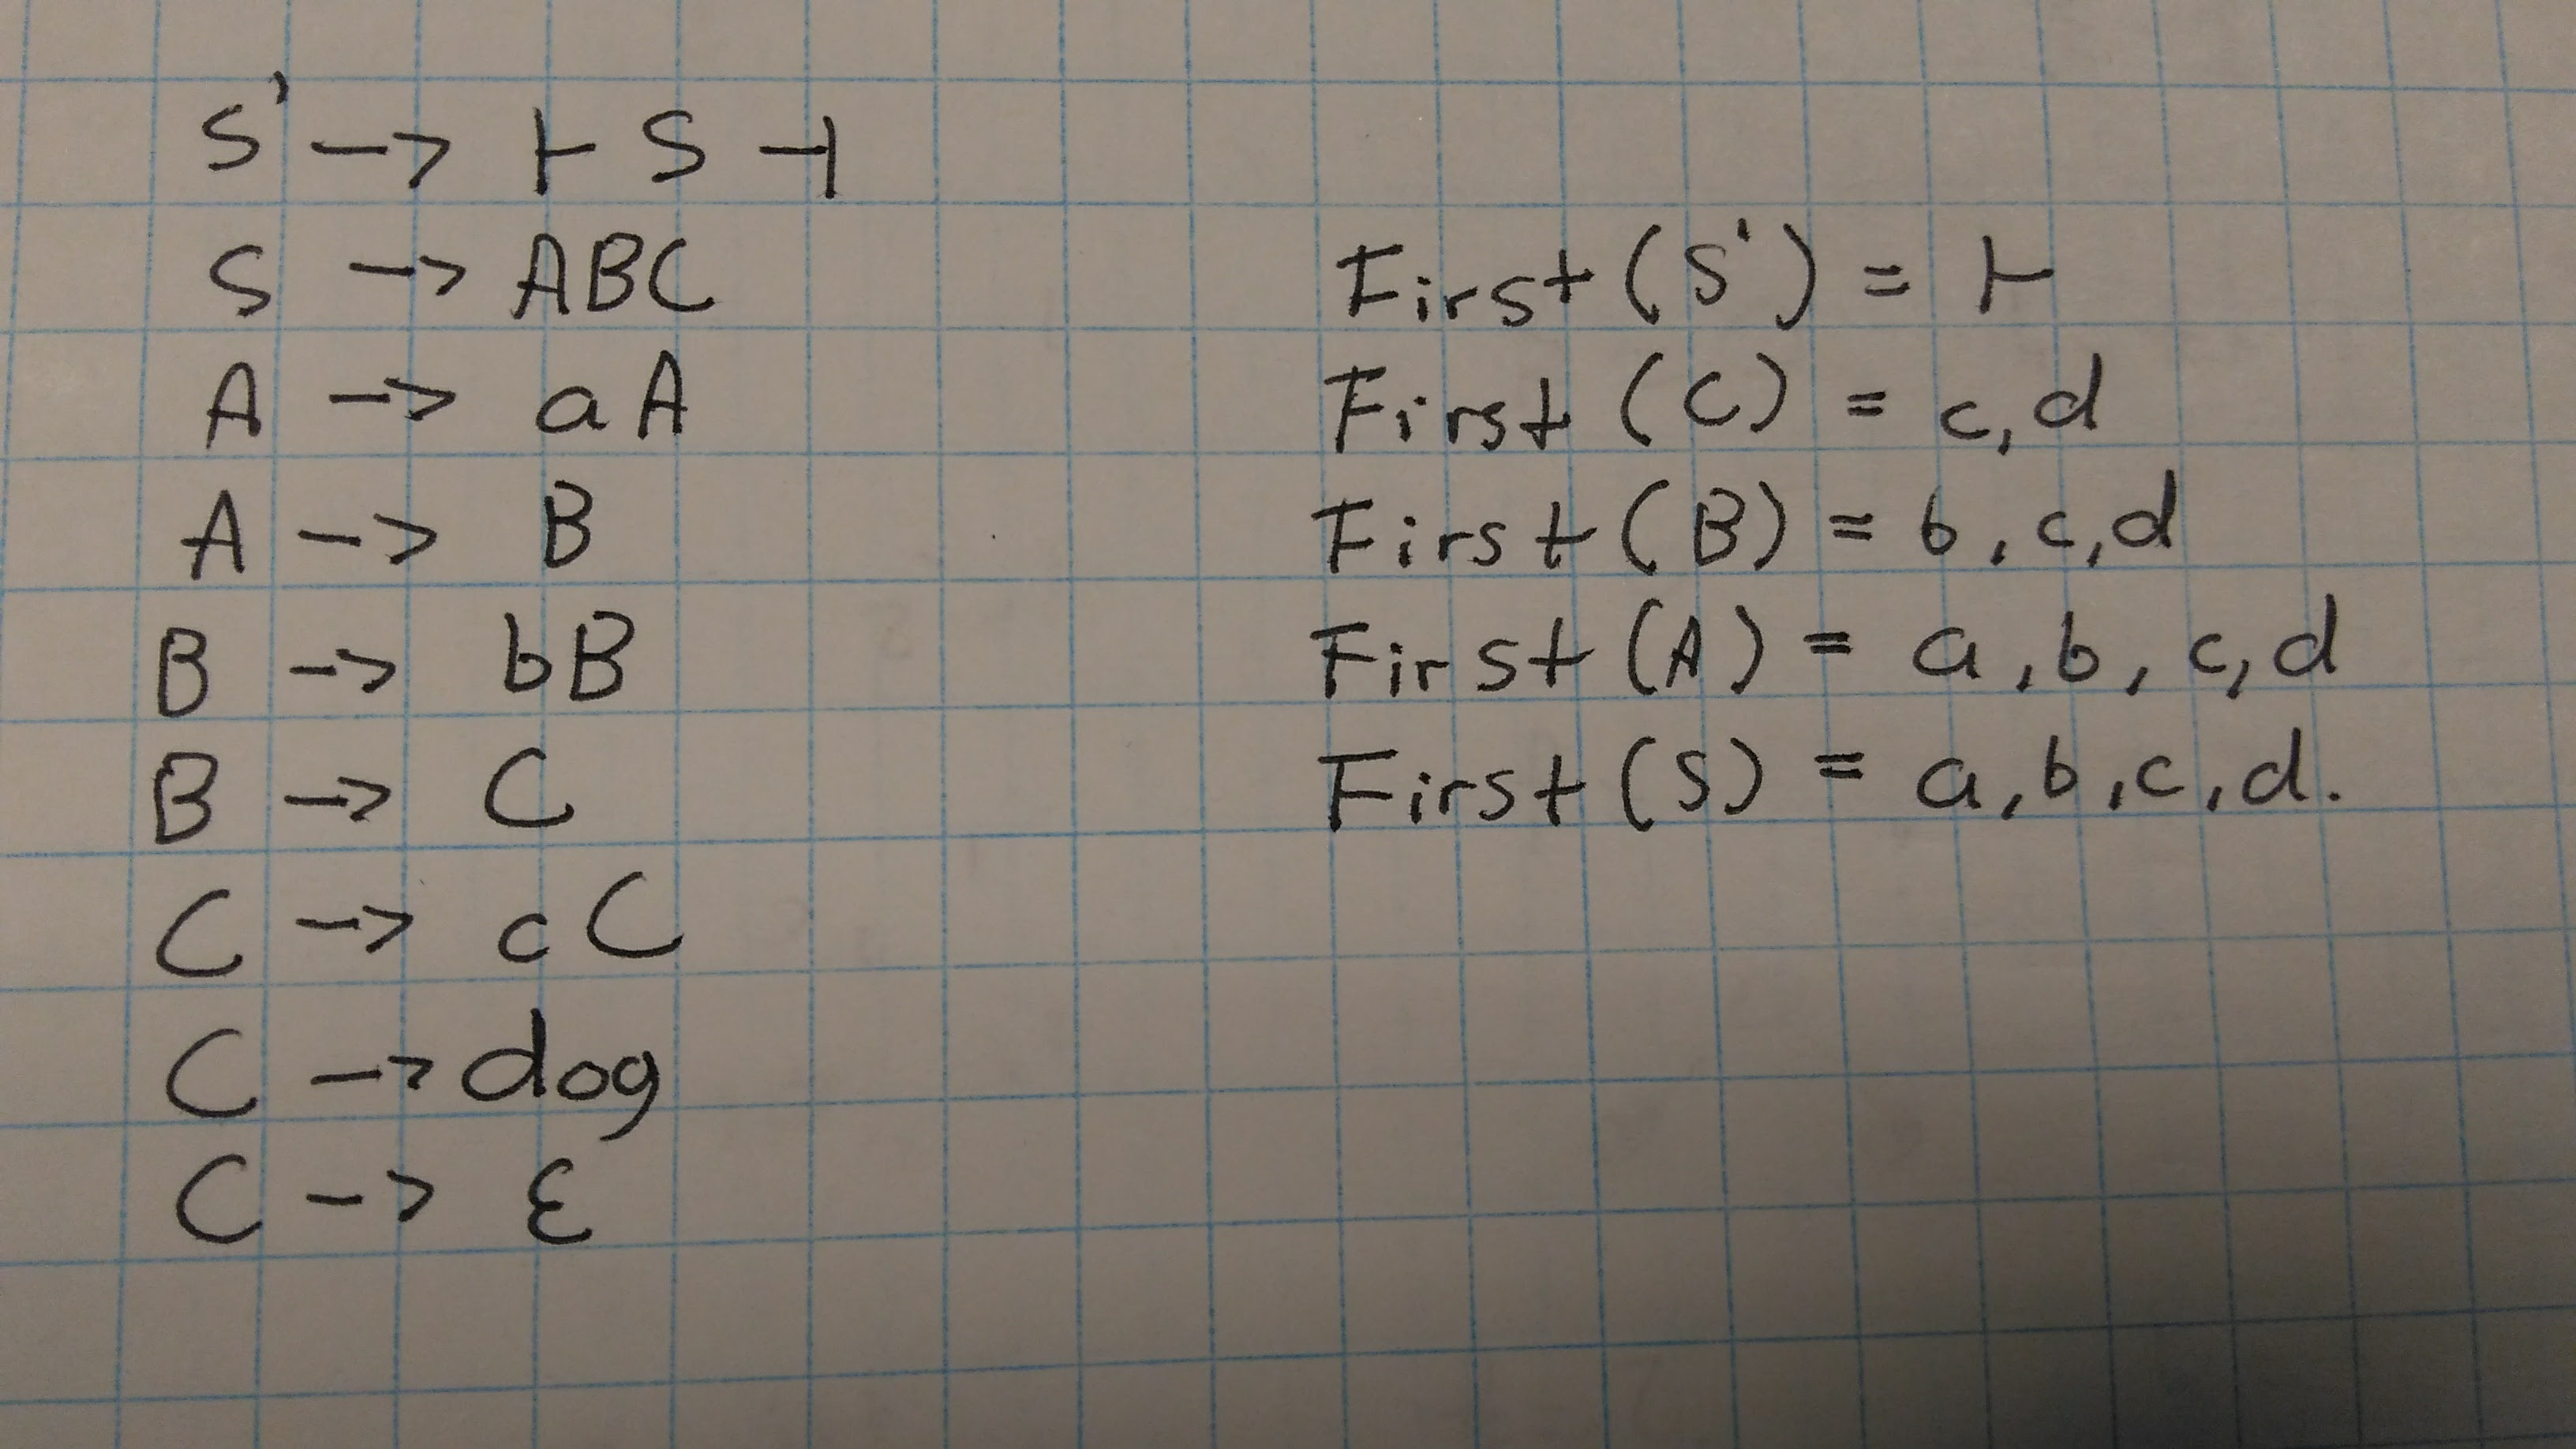
\includegraphics[scale=0.05]{first1.jpg}
\end{center}
\end{figure}
\item \texttt{follow($\alpha$)} returns the terminals that occur immediately following $\alpha$
\item \texttt{empty($\alpha$}: returns true if the given terminal or non-terminal $\alpha$ can disappear (i.e., $\alpha \rightarrow \varepsilon$). If $\alpha$ is a terminal, it returns false immediately, since terminals cannot disappear
\end{itemize}
%END%
\end{document}